\chapter{Generation of Computational Grid}\label{chapter-grid}

The computational grid is the basis of the grid-based numerical solver.
The simplest and most easily generated grid is a Cartesian grid (Figure~\ref{fig_grid_cart}), 
whose grid lines are parallel with Cartesian coordinate axes,
thus it can be easily generated by giving the triple value:
the starting point, number of points and the spacing interval.
But the Cartesian grid has difficulty to produce high accurate solution
if there is surface topography in seismic wave simulation.
For surface topography, a general cuvilinear grid system is more accurate (Figure~\ref{fig_grid_curv}).
Its grid lines conform with the surface topography,
thus the surface topography can be accurately represented by the grid.
CGFD3D supports both the Cartesian grid for high efficient simulation
and also the curvilinear grid for high accurate calculation with surface topography.

\begin{figure}[h!]
    \centering
    \subcaptionbox{Cartesian grid\label{fig_grid_cart}}%
        {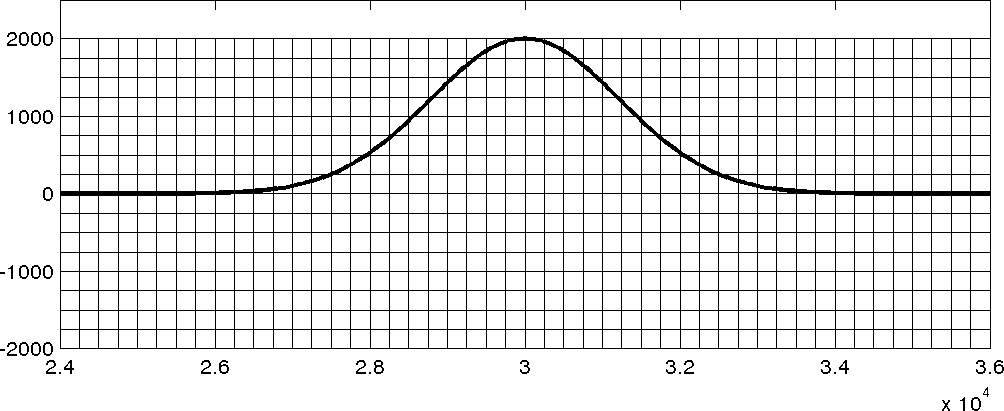
\includegraphics[width=0.4\textwidth]{grid_cart.png}}%
     \hspace{0.1\textwidth}
    \subcaptionbox{Curvilinear grid\label{fig_grid_curv}}%
        {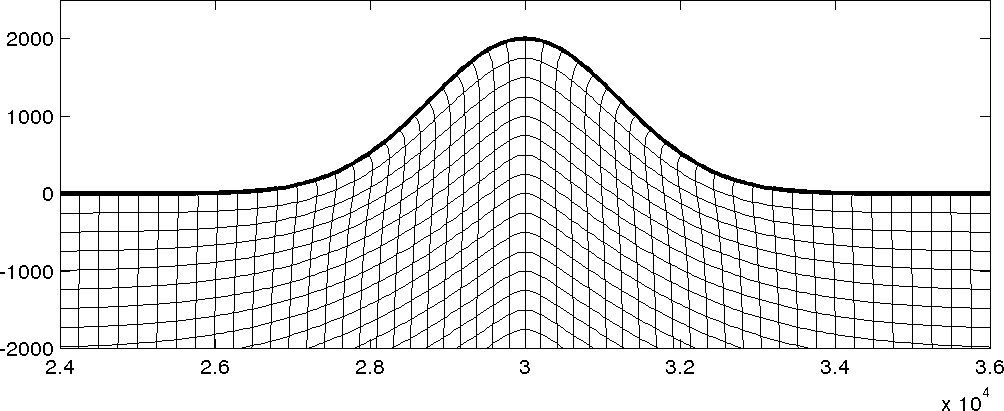
\includegraphics[width=0.4\textwidth]{grid_curv_bold.png}}%
    \caption{Computational grids}
    \label{fig_grid}
\end{figure}

%\begin{figure}
%    \centering
%    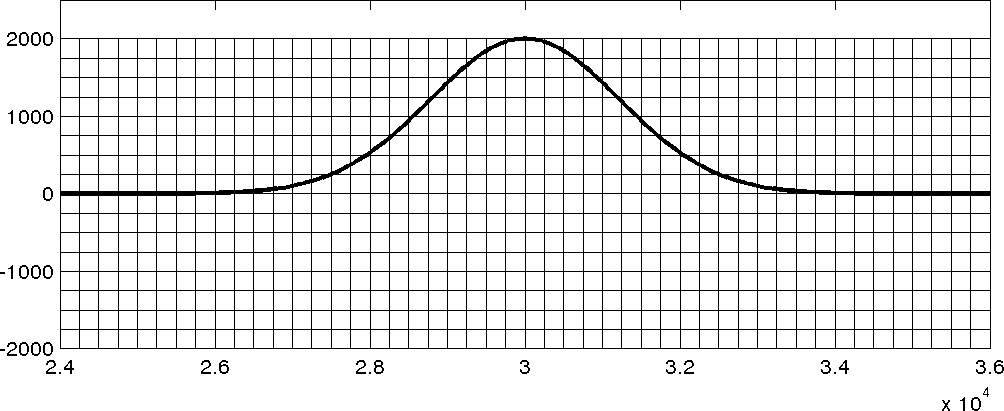
\includegraphics[width=0.5\textwidth]{grid_cart.png}
%    \caption{Cartesian grid with topographic surface plotted as bold line.}
%    \label{fig_grid_cart}
%\end{figure}
%
%%\begin{figure}
%%    \centering
%%    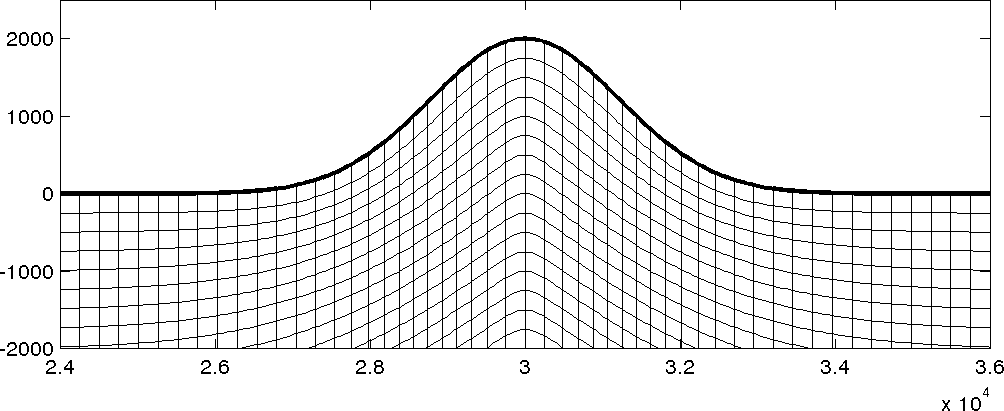
\includegraphics[width=0.5\textwidth]{grid_vmap_bold.png}
%%    \caption{Vertical deformated grid with topographic surface plotted as bold line.}
%%    \label{fig_grid_vmap}
%%\end{figure}
%
%\begin{figure}
%    \centering
%    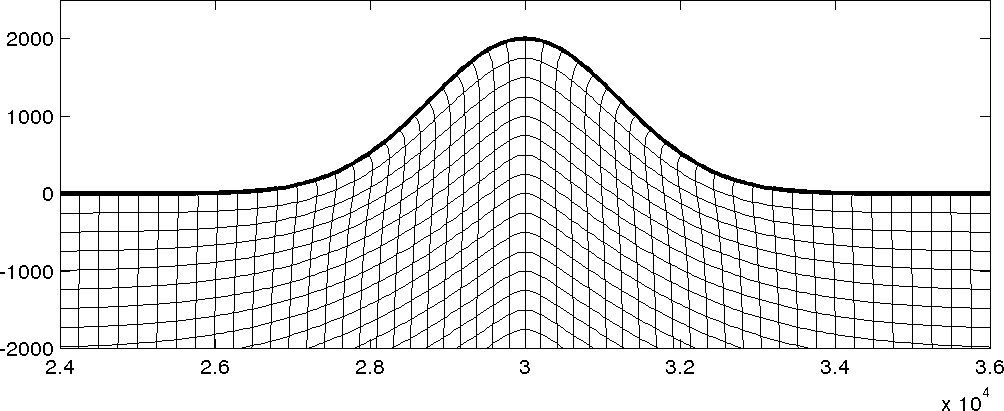
\includegraphics[width=0.5\textwidth]{grid_curv_bold.png}
%    \caption{General curvilinear grid with topographic surface plotted as bold line.}
%    \label{fig_grid_curv}
%\end{figure}


%===============================================================================
\section{Set Grid Parameters in Main Par} \label{sec_grid_json} 
%===============================================================================

\begin{lstlisting}[language=json,
 caption=Grid related parameters in .json,
 label={lst_grid_json},
 frame=tb]
  "grid_generation_method" : {
    "key name" : value
  },
  "is_export_grid" : 1,
  "grid_export_dir"   : "/home/user/prj/output",               
\end{lstlisting}

As shown in List~\ref{lst_grid_json}, user needs to set following parameters
related to the grid in .json file:
\begin{itemize}
  \item \verb|grid_generation_method|: \\
    how the grid is generated.
    There are current three possible methods:

    \begin{itemize}
      \item \verb|import|: \\
        import previoused generated curvilinear grid, 
        thus no need to re-generate grid for repeated run. 
        select this option and give the folder of the exported curvilinear grid, e.g.:  \\
        \verb|"import" : "/home/user/prj/grid"| 

      \item \verb|cartesian|: \\
        generate Cartesian grid, see next section for details.

      \item \verb|layer_interp|: \\
        generate general curvilinear grid, see later section for details.
    \end{itemize}

  \item \verb|is_export_grid|: \\
    if the coordiantes of the curvilinear grid are exported 
         for display purpose or reuse for later calculation without re-generateion of the curvilinear grid.
      \begin{itemize}
        \item 0: do not export,
        \item 1: export.
      \end{itemize}

  \item \verb|grid_export_dir|: \\
    set the output dir if \verb|is_export_grid : 1|.
\end{itemize}

%===============================================================================
\section{Generation of Cartesian Grid} \label{sec_cartesian} 
%===============================================================================

To use the Cartesian grid, we can simply set parameters in the .json file as List~\ref{lst_cart}.
The Cartesian grid needs following parametgers:
\begin{itemize}
  \item \verb|origin|: the x, y and z coordina of the first point,
  \item \verb|interval|: the x, y and z grid spacing. 
\end{itemize}

\begin{lstlisting}[language=json,
 caption={Example of Using Cartesian Grid in .json},
 label={lst_cart},
 frame=tb]
  "grid_generation_method" : {
      "cartesian" : {
        "origin"  : [0.0, 0.0, -5900.0 ],
        "inteval" : [ 100.0, 100.0, 100.0 ]
      }
  },
  "is_export_grid" : 1,
  "grid_export_dir"   : "/home/user/prj/output",               
\end{lstlisting}

%===============================================================================
\section{Generation of General Curvilinear Grid} \label{sec_curv} 
%===============================================================================

We implement a simplified curvilinear grid generation method:
input several topographic grid interfaces as intermidiate interfaces, 
then interpolate grid points between these grid interfaces
with given number of cells between interfaces, which we name as \verb|layer_interp| method.

\begin{lstlisting}[language=json,
 title={Usage Example of \texttt{layer\_interp} in .json},
 label={lst_curv},
 frame=tb]
  "grid_generation_method" : {
      "layer_interp" : {
        "in_grid_layer_file" : "/home/user/prj/input/test_grid.gdlay",  
        "refine_factor" : [ 1, 1, 1 ],
        "horizontal_start_index" : [ 3, 3 ],
        "vertical_last_to_top" : 0
      }
  },
  "is_export_grid" : 1,
  "grid_export_dir"   : "/home/user/prj/output",               
\end{lstlisting}

To use \verb|layer_interp| to generate the curvilinear grid,
we should provide following informations in the .json file (List~\ref{lst_curv}):
\begin{itemize}
  \item \verb|in_grid_layer_file|: \\
    the .gdlay file that represents the curvilinear grid using
      serveral topographic grid interfaces and number of cells between interfaces.
      Please see Section \ref{gridlayerinterp} of the file format description. 
  \item \verb|refine_factor|: \\
      The .gdlay file describes a whole curvinear grid with 
      pre-defined $nx,ny,nz$, number of grid points, and grid spacings.
      If we want to use a smaller grid spacing (denser grid) or larger grid spacing (corser grid),
      we can use this \verb|refine_factor| to change the grid density along different dimensions, e.g.,
      \begin{itemize}
        \item 1: no resampling;
        \item \texttt{2} or \texttt{3}: increase density by two or three times using interpolating;
        \item \texttt{-2} or \texttt{-3}: minus means downsampling by keeping points 
              every two or three points.
      \end{itemize}
      This parameter must be an integer and cannot be zero.
  \item \verb|horizontal_start_index| and \verb|vertical_last_to_top|: \\ 
    We can also use a smaller part of the total .gdlay grid in simulation .
    To do so, we need to tell the program the index of the starting point in the .gdlay to be used.
    Because CGFD3D uses a z-axis positive upward coordinate system, 
    the free surface is located at the end grid size with large number of index of the third dimension.
    Thus we specify the staring points for first and second dimensions through \verb|horizontal_start_index|, 
    while end points of the cut grid to that of the .gdlay through \verb|vertical_last_to_top|.
    E.g.,
    \begin{itemize}
      \item \verb|"vertical_last_to_top" : 0|: \\
          the last layer along 3rd-dim of the cut grid conincides with the free surface in the .gdlay.
      \item \verb|"vertical_last_to_top" : 40|: \\
          the last layer along 3rd-dim of the cut grid conincides with 
            the last 40 points along 3rd-dim in the .gdlay.
    \end{itemize}
    Note: if used with resampling by \verb|refine_factor|,
      there should be at least three points (for current DRP/opt MacCormack scheme) left
          outside the resulting computational grid as the ghost points,
          thus the \\
          \verb|horizontal_start_index| should be set to ensure this condition satisfied, e.g.:
    \begin{itemize}
      \item If you do not resample, the minimum value of \verb|horizontal_start_index| is 3;
      \item If you do two or three times  downsampling,
          the minimum value of \verb|horizontal_start_index| is 6 or 10;
      \item If you do two or three times interpolating,
        the minimum value of \verb|horizontal_start_index| is 2 or 1.
    \end{itemize}
\end{itemize}


%===================================================================
\section{Format of Grid Layer Interp File (.gdlay)} \label{gridlayerinterp}
%===================================================================

\begin{lstlisting}[language=bash,
    numbers=left, numbersep=5pt,numberstyle=\tiny\color{codegray},
    commentstyle=\color{codegreen},
    caption={Example of .gdlay file},
    label={lst_grid_gdlay},
    frame=tb]
     4
     43     10     10
      1      0      1
   126    106
     -300.00      -300.00     -5484.82
     -200.00      -300.00     -5483.59
     -100.00      -300.00     -5481.34
        0.00      -300.00     -5479.30
      100.00      -300.00     -5478.44
      200.00      -300.00     -5478.95
      300.00      -300.00     -5480.11
.
.
.
\end{lstlisting}

\begin{figure}
    \centering
    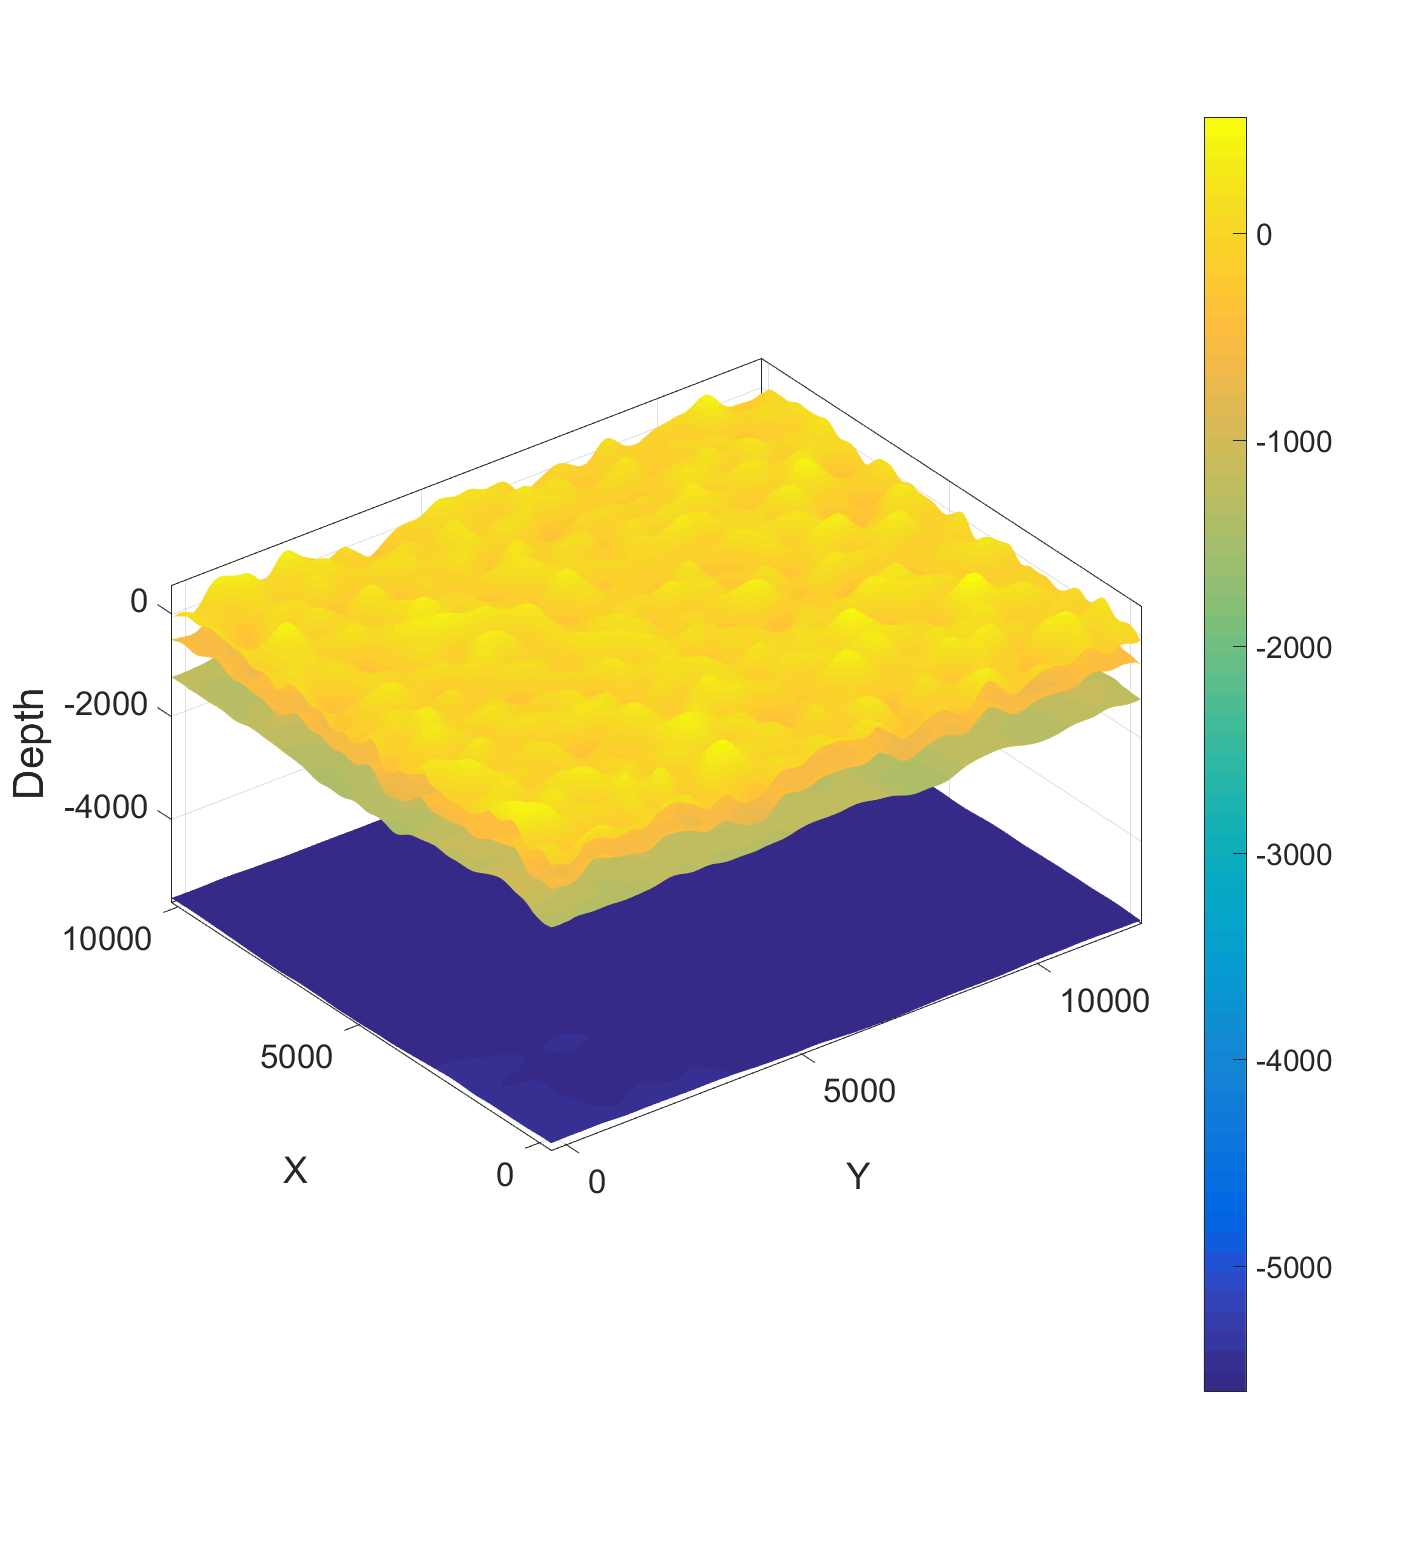
\includegraphics[width=0.8\textwidth]{gdlay_example.png}
    \caption{Examples of the grid interfaces in the .gdlay file.}
    \label{fig_gdlay}
\end{figure}


An example of .gdlay is shown in Listing~\ref{lst_grid_gdlay} and Figure~\ref{fig_gdlay}.
The detailed format of the .gdlay is:
\begin{itemize}
  \item The first line: \\
    the number of grid interfaces ($NI$, 4 in this example).
  \item The second line: \\
    number of cells of each layer
      (the space between two grid interfaces is called a layer).
    There are 43 cells between the 1st and 2nd grid interfaces,
      10 between 2nd and 3rd interfaces,
      10 between 3rd and 4th interfaces in this example.
 \item The third line: \\
   $NI-1$ int values to set if the grid spacing along the 3rd-dim is equal:
   \begin{itemize}
     \item 1: is equal, thus the grid spacing of the 3rd-dim is easily calculated by the two points
         of the grid interfaces in the .gdlay and number of cells of this layer specified in previous line.
     \item 0: not equal or should smoothly vary from 
          the grid spacing of the above grid interfaces to that of lower grid interfaces.
   \end{itemize}
   The variation of the grid spacing between grid layers should be as smooth as possible.
   The vartions of the horizontal grid space is determined by the input grid interfaces in the .gdlay,
    while the variation of the 3rd-dim is affected by values of this line.
   CGFD3D will first generate the grid of the grid layers with equal grid spacing, 
   then generate rest grid between these equal-spacing layers.
   Thus any layer of ``0'' equal value, should have both ``1''  layers above and below it.
  \item The fourth line: \\
    two int values $NX$ and $NY$,
        the number of horizontal grid points of each grid interfaces 
         of this .gdlay file. The numbers are same for all the grid interfaces.
         %thus are given once in this line for all the interfaces.
  \item 
    Rest are the X, Y and Z coordinates of each grid point per line.
    The order of the grid points is:
      1st-dim, then the 2nd-dim of the first grid interface (the bottom one as the z-axis upward positive);
      then those of the 2nd grid interfaces, etc,
    which can can be expressed by the following pseduo code:
\begin{verbatim}
    for (int ilay = 0; ilay < NI; ilay++) {
      for (int j = 0; j < NY; j++) {
        for (int i = 0; i < NX; i++) {
          fscanf(fp,"%g %g %g", &xcoord, &ycoord, &zoord);
        }
      }
    }
\end{verbatim}

\end{itemize}

We provide some examples of matlab scripts to generate .gdlay under the \texttt{example/prep\_grid} directory.

%\subsection{Example}
%
%A model with a horizontal interface can be given as:
%
%\begin{lstlisting}[language=python, title=test.gdlay, frame=tb]
%  4
%  20    10    20
%  1       0     1    
% 100  100
%    100.0    100.0  -5000.0   
%    200.0    100.0  -5000.0
%    300.0    100.0  -5000.0
%    400.0    100.0  -5000.0
%     ...      ...      ... 
%\end{lstlisting}
%The given interface model have 4 interfaces. \\
%There are 20 cells between the first interface and the second interface; there are 10 cells between the second interface and the third interface; there are 20 cells between the third interface and the fourth interface. The first interface is the deepest underground interface, and the last is the free surface interface. \\
%The cell spacing between the first interface and the second interface are equal; the cell spacing between the third interface and the fourth interface are equal; the cell spacing between the second interface and the third interface is gradual.\\
%The number of interface grids in X is 100 and the number of interface grids in Y is 100. The number of interface grids in Z is 51 ( 4+(20-1)+(10-1)+(20-1) ). \\
%
%The given interface model size is \texttt{100*100*51} .
%In fact, the largest model area we can calculate is \texttt{(100-2\*fdx\_nghosts)*(100-2\*fdy\_nghosts)*(51-fdz\_nghosts)}. 
%(In this program, these parameters \texttt{fdx\_nghosts, fdy\_nghosts, fdz\_nghosts} are colonization 3). So the largest model area we can calculate is \texttt{94*94*48}.  \\
%
%(1) Example of the maximum area we can calculate without resampling: \\
%\texttt{number\_of\_total\_grid\_points\_x = 94}, \\
%\texttt{number\_of\_total\_grid\_points\_y = 94}, \\
%\texttt{number\_of\_total\_grid\_points\_z = 48},  \\
%\begin{lstlisting}[language=python, title=run\_test.sh, frame=tb]
%      "layer_interp" : {
%        "in_grid_layer_file" : "$EXEC_DIR/test/test_grid.gdlay",  
%        "refine_factor" : [ 1, 1, 1 ],
%        "horizontal_start_index" : [ 3, 3 ],
%        "vertical_ToFreeSurf_resample_index" : 0
%      }        
%\end{lstlisting}
%the calculation area index range of x is \texttt{3->96}, \\
%the calculation area index range of y is \texttt{3->96}, \\
%the calculation area index range of z is \texttt{3->50}. \\
%In the x direction, ghosts points is \texttt{0->2}, and \texttt{97->99}, \\
%in the y direction, ghosts points is \texttt{0->2}, and \texttt{97->99}, \\
%In the z direction, ghosts points is \texttt{0->2}.\\
%
%(2) Example of the partial area we can calculate without resampling: \\
%\texttt{number\_of\_total\_grid\_points\_x = 50}, \\
%\texttt{number\_of\_total\_grid\_points\_y = 40}, \\
%\texttt{number\_of\_total\_grid\_points\_z = 25}.  \\
%\begin{lstlisting}[language=python, title=run\_test.sh, frame=tb]
%      "layer_interp" : {
%        "in_grid_layer_file" : "$EXEC_DIR/test/test_grid.gdlay",  
%        "refine_factor" : [ 1, 1, 1 ],
%        "horizontal_start_index" : [ 20, 35 ],
%        "vertical_ToFreeSurf_resample_index" : 10
%      }        
%\end{lstlisting}
%the calculation area index range of x is \texttt{20->69}, \\
%the calculation area index range of y is \texttt{35->74}, \\
%the calculation area index range of z is \texttt{16->40}. \\
%In the x direction, ghosts points is \texttt{17->19}, and \texttt{70->72}, \\
%in the y direction, ghosts points is \texttt{32->34}, and \texttt{75->77}, \\
%In the z direction, ghosts points is \texttt{13->15}, and \texttt{41->42}. \\

%number\_of\_total\_grid_points\_x

